\documentclass[pdflatex,sn-nature]{sn-jnl}

\usepackage{graphicx,booktabs,array,tabularx,amsmath,amssymb,xspace,adjustbox}
\usepackage{xurl}
\usepackage[expansion=false]{microtype}
\graphicspath{{images/}{./}}
\emergencystretch=2em
\raggedbottom
\newcommand{\allow}{\textsc{Allow}\xspace}
\newcommand{\block}{\textsc{Block}\xspace}
\newcommand{\clarify}{\textsc{Clarify}\xspace}

\begin{document}
\title[Request-grounded authorization for agents]{NiyamTrace-X: An Agent-Based Multilingual Tool for Evaluating Request-Grounded Authorization}
\author[1]{\fnm{Agasthya Anirudh} \sur{Badampudi}}
\author[1]{\fnm{Sri Pranav} \sur{K}}
\author*[1]{\fnm{Vijayarajan} \sur{V}}\email{vijayarajan.v@vit.ac.in}
\affil[1]{\orgdiv{School of Computer Science and Engineering},\orgname{Vellore Institute of Technology},
\orgaddress{\city{Vellore},\state{Tamil Nadu},\country{India}}}
\abstract{NiyamTrace-X links instructions in multiple languages to database changes via explicit request anchors, policy constraints and mediated execution. We tested the system in three different ways: deciding on reference verdicts, deciding paired effects that are allowed and native SQLite commits. On a frozen generated holdout of 2,000 requests per model, request anchoring with clarification recovery resulted in final verdict accuracies of 99.85\% for Qwen3.5-122B and 99.80\% for GPT-OSS-120B, with no unsafe final verdicts observed. In a paired 360-request experiment, independent interpretation intersection did not remove any additional unauthorized effects. For Granite, it dropped the accuracy from 93.33\% to 80.00\% and the exact authorized completion from 152/162 to 104/162. A known-candidate control answered all the 48 native probes correctly and also completed all the 12 authorized actions. Live Qwen2.5-3B did only 3/12 authorized actions; however, it also performed three explicitly prohibited archives that changed five invoice rows. Granite-3.3-2B did not do any. High accuracy of reference decisions did not prove safety in the independently evaluated native pipeline, which used different models, interfaces, and authorizations, which means that semantic authorization checking is a must before a database write.
 It also argues for reporting verdict accuracy, fidelity to the request, committed effects, and authorized task completion together.}
\keywords{language model agents, authorization, multilingual evaluation, semantic contracts, tool execution, agent safety}
\maketitle
\section{Introduction}

It is possible that a procurement manager who is allowed to archive invoices can still direct an agent to keep them unchanged. All the conditions such as the role being valid, the vendor identifier being valid, and the proposed database operation being properly formed might be met. However, the instruction does not authorize any archival. In fact, a policy engine receiving only the agent's positive interpretation might end up approving exactly the action that was prohibited by the user. For agents who can affect the external state, this discrepancy between what the role allows and what the user authorizes becomes very significant.

With three experiments involving different units of evaluation, we manage to answer the questions above. Frozen ablation is a method of isolating anchoring and clarification recovery on 2,000 requests per large checkpoint. Paired effect comparisons, on the other hand, not only change the authorization method but also keep the preferred proposal fixed. Then, auditing of committed changes to a database against request-grounded expectations is performed in a native SQLite experiment. A known-candidate control is a technique used to separate the broker's ability to execute an authorized operation from the model's ability to provide the correct semantic inputs. In essence, we question whether anchoring enhances controlled verdicts, whether independent candidates increase safety without completely removing useful actions, and whether live model outputs maintain a request through commit. Since these cohorts measure different outcomes, they are not pooled.


\section{Related work and research gap}
Toolformer focuses on learning when language model should call an API, while ReAct mixes reasoning with performing actions \cite{toolformer2023,react2023}. API-Bank, ToolLLM and Gorilla broaden their evaluation or training to more extensive API environments \cite{apibank2023,toolllm2024,gorilla2024}. These papers show that an agent can accurately use tools and finish tasks. Authorization adds three questions: who is the requester's identity that supports the action, what effects the request allows, and whether those limits survive through the ‌commit.

Benchmarks for agent safety address a number of interconnected failure modes. ToolEmu analyzes unsafe behaviors in simulated environments; AgentDojo and InjecAgent rely on the evaluation of attacks by means of untrusted external contents; Agent Security Bench covers a broad scope of agent failure modes \cite{toolemu2024,agentdojo2024,injecagent2024,asb2025}. Besides the text generation failure modes, function-calling and interactive-task benchmarks like BFCL and $\tau$-bench show more failure cases \cite{bfcl2025,taubench2025}. They encourage looking at the action path instead of depending only on a tool-call score. Their as-is scores cannot be used to assess an authorization mechanism that was not included in the tested trajectories.

Current security measures are implemented in a variety of locations along the action path. Through indirect prompt injection, instructions can be provided via the data that the application is handling \cite{greshake2023}. IsolateGPT divides the aspects of running a program, CaMeL restricts the execution of agents by splitting control and data-flow, and AttriGuard evaluates whether there is a causal justification for the proposed tool uses \cite{isolategpt2025,camel2026,attriguard2026}.

While ToolSafe brings in-level approaches to safety, SAGA controls the agent's identity, delegation, and access aspects \cite{toolsafe2026,saga2026}. AgentSpec and truly capable systems communicate limitations through runtime rules or programming-language capabilities \cite{agentspec2026,trackedcaps2026}. NiyamTrace-X looks at the conversion of the request into the effect bearing contract, and then whether the accepted contract actually limits the executed changes.

Multilingual languages make the conversion more difficult to evaluate. Lost in Execution examines cross-language tool-calling errors dependent on execution, while TUCAN creates resources for non-English function calling \cite{lostexecution2026,tucan2026}. MASSIVE and MTOP are public language-understanding datasets giving the possibility of testing an extractor independently of an enterprise authorization label \cite{massive2023,mtop2021}. The difference is significant because the error rate of an intent classifier is not only the rate of unauthorized writes but also a measure of successful authorized execution.

The security principles of this design went beyond the creation of language-model agents. Least privilege grants minimal rights, confinement restricts the spread of effects, and integrity policies limit the occurrence of sensitive transitions \cite{saltzer1975,lampson1973,clarkwilson1987}. Execution monitors and edit automata serve the purpose of formalizing the way enforcement is done over represented actions \cite{schneider2000,ligatti2005}. Their assurances depend on what is represented to the monitor. For an agent, the represented action is deduced from a request, and even a seemingly well-scoped operation can still go against that request. Hence, compliance to the policy and compliance to the request should be gauged independently.

This literature results in a three-part test:

1) Was the request interpreted correctly? 2) Is the effect proposed by the request in line with the policy? 3) Does the committed state change correspond to the authorized effect? We do not infer a tool-call success as evidence of authorization, rather, we directly measure each part.

\section{NiyamTrace-X architecture}

Initially, NiyamTrace-X will generate candidate contracts listing the possible effects for each request. The implementation of a proposed action is constrained not only to the effects of those contracts that uphold the principal's policy but also to the effects of principal's policy. The use of explicit anchors enables a proposal to be compared with the original request details, whereas the candidate intersection tests whether independent interpretations may further reduce an uncertain scope. The containment argument is only valid if the language front end maintains the relevant meaning and the native executor mediates every resulting effect. Our research looks into these two aspects along with even more concrete boundaries of making sure the relevant meaning is preserved and every resulting effect is mediated.


The reference representation records an action, an entity, a month, a year, a value, a currency, a quantifier, a scope and negation, along with clarification and disagreement information.

Define $I(u)$ as the set of candidate contracts kept for request $u$, $P(p,s)$ as the rights that principal $p$ is allowed in state $s$, and $\widehat{E}(C,s)$ as the rights derived from contract $C$.

The correct authorized set at that point is
\begin{equation}
A(u,p,s)=
\begin{cases}
\varnothing, & I(u)=\varnothing,\\
P(p,s)\cap\displaystyle\bigcap_{C\in I(u)}
\widehat{E}(C,s), & \text{otherwise}.
\end{cases}
\label{eq:authorization}
\end{equation}
The system consists of a language front end, an authorization boundary and an execution boundary. The front end extracts an intended operation and its slots. The reference decision path checks only the explicit request anchors against the proposed contract prior to policy evaluation and, in one variant, intersects the independent candidate effects. The evaluated native gateway on the other hand, checks the model's extracted proposal against trusted role and tenant information, policy constraints and retrieved policy evidence; it does not independently derive explicit negation from the request. A native proposal that is permitted obtains an effect-bound capability. Within a SQLite transaction, the broker verifies the capability and database state, executes the operation and compares the actual row changes with the certified effect. Equation~\ref{eq:authorization} represents the rule grounded in the request-product, not an assurance that every native extraction complies with it.

\section{Methods}
\subsection{Design and evidence selection}
Our study involves an examination of ERP requests that were generated, synthetic SQLite fixtures as well as a few public language-understanding examples chosen for their representativeness. We are not conducting here any real financial transaction. Role and tenant information that is considered trustworthy is kept separate from the textual content of the request. The threat model covers mismatched selectors, missing authorizations, and forgetting prohibitions, but it does not include scenarios like privileged Python code execution, signing-key leakage, distributed concurrency, and external enterprise connectors.

We looked at the retained archives, run manifests, scorer outputs, and database snapshots to make sure that the results we selected were after reconciliation. Duplicate exports cannot be used to increase the size of a cohort; runners that failed and the counts of unsupported headlines do not provide any estimate. Private participant requests are excluded from
the reported analyses, and the recoverable
inventory is not an exhaustive record of all
project artifacts.

\subsection{Reference protocol and pseudocode}
The frozen corpus comprises 500 semantic groups expressed in English, Romanized Hindi, Romanized Telugu, and Telugu script: 2,000 requests per checkpoint. Eight relation families loosely equivalent, narrower, broader, negated, entity-, time- and value-shifted, and ambiguous requests. Expected verdicts are 504 \allow, 1,248 \block and 248 \clarify. Programmatic labeling follows sampled relation and authority fixture. Development and holdout sets are disjoint and both belong to the same generator family, forming internal validation. Qwen3.5-122B-A10B-FP8 and GPT-OSS-120B have been used via vLLM in an AMD Instinct MI300X setup. Reproducibility log captures revisions, client, prompt, schema, scorer, execution, and content hash values. Qwen determines 1,042 outputs to be cached while GPT-OSS identifies zero. We analyze saved outputs without a goal of conducting two-model inference experiment anew or conducting latency comparison. Base, anchor only, and clarification only verdicts are reconstructed from saved policy, anchor, and recovery flag values; full verdict is captured through final saved result.

The reference authorization pseudocode is:
\begin{enumerate}
    \item Extract candidate contracts; reject malformed candidates.
    \item Block an explicitly prohibited write; clarify unresolved critical scope.
    \item Retain contracts consistent with explicit request anchors.
    \item Permit no write when no contract remains; otherwise intersect candidate effect sets with policy-permitted effects using Equation~\ref{eq:authorization}.
    \item Allow only proposals contained in that set, without widening it for completion.
\end{enumerate}

Clarification recovery only discards an unnecessary prompt after compatible effects survive the checks. Condition for containment is that the interpretations are faithful and complete, the effect compilation is conservative, the policy is current, and the mediation is complete. A language model that satisfies the conditions cannot be proved solely by set inclusion. An unnecessary candidate can remove an intended action.

\subsection{Paired and native protocols}

Qwen2.5-3B-Instruct and Granite-3.3-2B-Instruct each serve as primary and secondary interpreter. Each of the two primary-model directions utilizes 240 controlled realizations from 80 groups and 120 minimal-pair realizations from 20 groups, in the languages of English, Romanized Hindi and Romanized Telugu. Six methods---raw, policy-only, anchors, single-best, independent-only and full---reuse each preferred proposal. The 4,320 method rows represent 720 model--request pairs, not independent requests. A reference SQLite oracle compares row changes with generated authorized sets. Broad \texttt{ALLOW\_ALL} fixture permissions actually test set operations rather than suggest an unrestricted deployment. A retest only identifies 48 regressions previously found in Granite; it is not a new full-cohort replication.

The native corpus intersects three vendors, two invoice months, two language conditions and four request families. Twelve requests are \texttt{ALLOW}, twelve use unauthorized viewer roles, twelve omit the year and twelve explicitly forbid archival: twelve \texttt{ALLOW}, twenty-four \texttt{BLOCK} and twelve \texttt{CLARIFY} expectations. Six vendor--month groups share templates. Local generation employs FP16 on a Tesla T4, deterministic decoding and a 512-token cap. Both checkpoint changes and source, policy and prompt fingerprints are kept. These units pinpoint the version tested, not an externally verified runtime.


Messages contain requests and trusted fixture context but not gold label annotations. The validation process consists of identifying intentions and slots, checking that month and year can be expressed as integers, and checking that the numeric confidence is within a certain threshold; no normalization happens after the fact. Numeric confidence is extraction metadata,
not a calibrated safety probability
\cite{uncertaintyagent2024}. Schema has decision, intent, slots and confidence but not negation slot. Prohibitions should lead to unknown intent and blocked decision. The native pipeline executes the compiled proposal without model decision being an enforced veto.

Policy-document retrieval uses token-set Jaccard and fuzzy partial-string similarity combination at equal weights, returns up to three allowed document chunks. Rule engine verifies support for proposed intent and role; it doesn't recover request polarity by itself. Gate checks cover role, scope, tenant, target, time, attributes, cardinality and evidence. Proposals agreed upon get HMAC-bound capabilities with arguments, authorization context, policy, predicted delta, nonce and expiry. During a transaction, broker verifies both capability and state, performs operation, compares real and certified changes, and records consumed capabilities. Signing keys protection and faithful semantic inputs are still correctness factors.


Every accepted extraction is provided with a new seeded database. Full before/after logical states and last SQLite files are connected to execution events and capability consumption. The 100\% positive completion means that each invoice that is originally OPEN and within the authorized scope must be changed to ARCHIVED, without perform any other business change. Partial results, no changes, denials, and incorrectly formatted outputs result in failure to complete.

Nonce records are also tallied separately. A known-candidate control reuses all 48 requests without model inference. Eighteen live and forty-eight control database pairs were independently verified; source tests remain separate coverage evidence.

\subsection{Metrics, language diagnostic and statistics}
Let $G_u$ be the generated authorized business-effect set and $E_u$ the observed changes. With $N$ attempted requests,
\begin{equation}
C_+=\frac{\sum_{u:G_u\ne\varnothing}\mathbf{1}\{E_u=G_u\}}{|\{u:G_u\ne\varnothing\}|},\qquad
R_{\mathrm{unsafe}}=\frac{\sum_u\mathbf{1}\{E_u\setminus G_u\ne\varnothing\}}{N}.
\label{eq:outcomes}
\end{equation}
Multiple changed rows count as one unsafe request; row totals are also reported. Verdict-only studies have no executed-effect risk estimate. Exact verdict accuracy retains all attempts, including output failures. Frozen semantic correctness additionally checks eight fields, clarification and disagreement; eight-field exact match is separate.

The selected twelve-class MASSIVE diagnostic uses twenty-four test items each in English, Hindi, Kannada, Tamil and Telugu; MTOP uses twenty-four English and twenty-four Hindi items \cite{massive2023,mtop2021}. Models choose among within-language prototypes. Dataset paths, content hashes, class mappings and predictions are retained; the revision name \texttt{refs/convert/parquet} is mutable. This is neither full-label-space leaderboard evaluation nor an ERP authorization test.

We use 10,000 whole-semantic-group percentile bootstrap draws, seed 20261013. Frozen groups have equal size. Paired groups have three or six realizations, so case-weighted differences are primary and equal-group means are sensitivity estimates. Unclustered McNemar values are not inferential evidence. Native and public-language results are descriptive. Under independent, exchangeable group sampling, the illustrative one-sided 95\% zero-event bound is $1-0.05^{1/g}$: about 0.80\% for 374 eligible frozen groups. This does not establish deployed population risk. Cohorts and measured boundaries are never pooled.

\subsection{Research ethics and data provenance}
No participants were recruited for the reported analyses. Private participant requests are excluded and not redistributed; public datasets retain their original terms. Findings were checked against retained records, and references against published records.
\subsection{Exploratory schema-corrected effect replay}
An additional retrospective audit used 240 saved proposals generated by Qwen2.5-3B-Instruct and Granite-3.3-2B-Instruct, with 120 requests for each model. The requests were produced from 30 generated task families, each expressed in English, Hindi, Telugu and Romanized Telugu. Within each model's 120 cases, 16 were labelled \allow, 68 \block and 36 \clarify. Only four underlying families were authorized; the remaining 26 non-\allow families account for 104 language realizations. These are scripted templates, not independently adjudicated natural user instructions.

The first run (NTX-24) evaluated the original strict proposal parser. NTX-24B did not generate new model responses. Instead, it reinterpreted the same frozen raw responses using a defined typed parser that recognizes supported resource-ID prefixes, numeric and named-month representations and required fields, without consulting hidden outcome labels. We compared the original and corrected parsers on the same cases, then replayed proposals against isolated before-and-after SQLite states under four reference policies: ungated model-only execution, role/scope validation, request-text grounding, and request-text grounding with a transaction-bound certificate and effect verifier. All reported committed effects are differences in business-state rows, not simply permission verdicts.

A separate scripted mechanism test inserted an unexpected extra mutation into otherwise authorized reference operations. Its 24 paired task-language probes came from only six authorized task families; each probe was tested under both the text-grounded and transaction-verifying reference arms. This experiment contains no additional model inference and is analysed independently of the 240-response cohort. The reference implementations are not the integrated native NiyamTrace-X production executor.

\section{Results}
\subsection{Exploratory parser and executed-effect audit}
The strict parser accepted complete proposals for only 13/120 Qwen requests and 0/120 Granite requests. On the same saved generations, the corrected typed parser accepted 77/120 complete proposals for each model. These are changes in the usability of existing proposals, not evidence of better model inference. For Qwen, seven previously accepted proposals became incomplete under the corrected required-field checks, even as other rejected typed proposals were recovered.

\begin{table}[htbp]
\centering\footnotesize\setlength{\tabcolsep}{3.5pt}
\caption{Retrospective typed-parser replay of 120 frozen generations per model. Unsafe effects count actual mutations among 104 non-\allow requests; completion counts exact intended effects among 16 authorized requests. The zero values are observations, not population guarantees.}
\label{tab:ntx24b}
\begin{tabular}{llrrr}
\toprule
Model & Reference arm & Unsafe /104 & Complete /16 & Exact /120 \\
\midrule
Qwen & Model only & 61 & 13 & 56 \\
Qwen & Role/scope & 25 & 13 & 92 \\
Qwen & Text grounded & 0 & 13 & 117 \\
Qwen & Transaction verified & 0 & 13 & 117 \\
\midrule
Granite & Model only & 60 & 13 & 57 \\
Granite & Role/scope & 25 & 13 & 92 \\
Granite & Text grounded & 0 & 13 & 117 \\
Granite & Transaction verified & 0 & 13 & 117 \\
\bottomrule
\end{tabular}
\end{table}

\subsection{Language-stratified parser recovery and executed effects}\label{sec:ntx24b_languages}
The corrected-parser replay also permits a matched comparison by language form (Table~\ref{tab:ntx24b_languages} and Figure~\ref{fig:ntx24b_languages}). Each model saw 30 requests per language, comprising four gold-\allow and 26 non-\allow realizations. Parser acceptance concerns the completeness of a generated tool proposal; authorized completion and unauthorized commits instead concern the resulting SQLite business state. We keep these endpoints separate because just a parsing failure can give the appearance of conservative authorization.

\begin{table}[htbp]
\centering\scriptsize\setlength{\tabcolsep}{3pt}
\caption{Exploratory NTX-24B results by language form, all based on the same frozen NTX-24 model generations. Parser entries show strict $\to$ corrected complete proposals out of 30. Completion is under request-text grounding among four authorized cases; unsafe counts show ungated $\to$ grounded committed effects among 26 non-\allow cases. Each language shares task families with other language forms.}
\label{tab:ntx24b_languages}
\begin{tabular}{llccc}
\toprule
Model & Language & Parser /30 & Complete /4 & Unsafe /26 \\
\midrule
Qwen & English & 2$\to$23 & 4 & 16$\to$0 \\
Qwen & Hindi & 9$\to$19 & 3 & 16$\to$0 \\
Qwen & Telugu & 2$\to$18 & 3 & 15$\to$0 \\
Qwen & Romanized Telugu & 0$\to$17 & 3 & 14$\to$0 \\
\midrule
Granite & English & 0$\to$20 & 4 & 16$\to$0 \\
Granite & Hindi & 0$\to$17 & 3 & 13$\to$0 \\
Granite & Telugu & 0$\to$26 & 4 & 19$\to$0 \\
Granite & Romanized Telugu & 0$\to$14 & 2 & 12$\to$0 \\
\bottomrule
\end{tabular}
\end{table}

\begin{figure}[htbp]
\centering
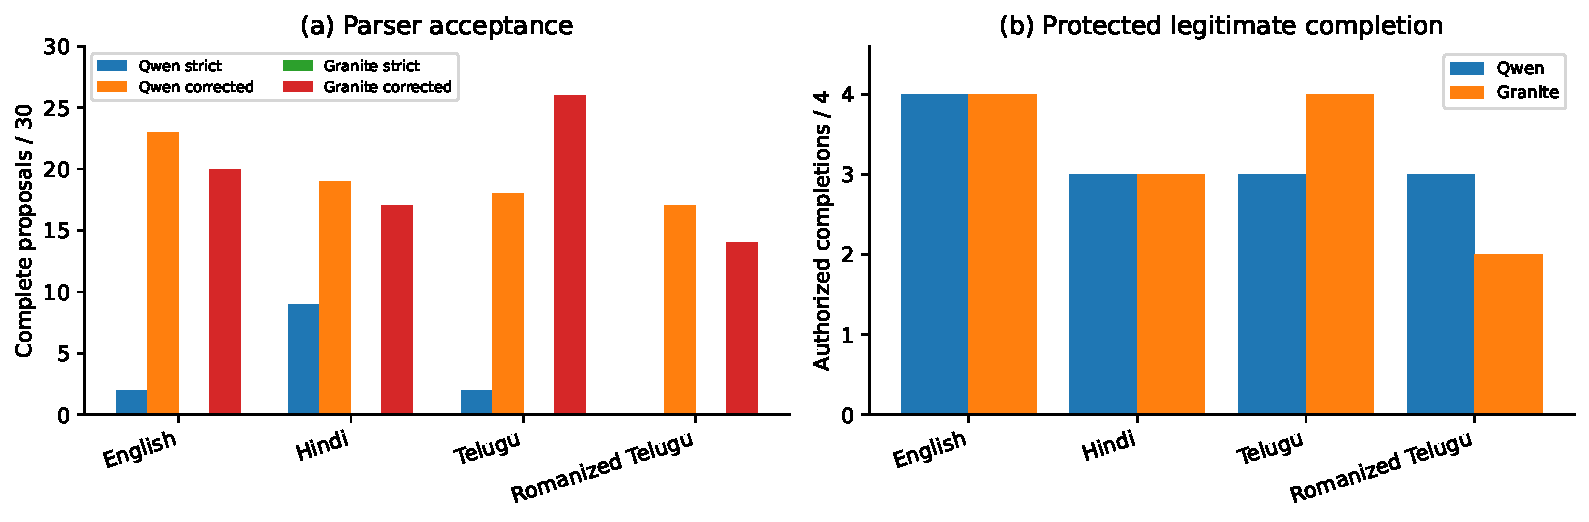
\includegraphics[width=\linewidth]{figure_6_ntx24b_by_language.pdf}
\caption{Language-stratified outcomes on the NTX-24/24B frozen template cohort: complete-proposal acceptance before and after typed normalization (left) and legitimate task completion after request-text grounding (right). Each plotted language has only four authorized realizations per model. Zero observed unauthorized commits under grounding are given separately in Table~\ref{tab:ntx24b_languages}; bars are not population safety guarantees.}
\label{fig:ntx24b_languages}
\end{figure}

English authorized cases completed for both models (4/4), while Granite completed 2/4 Romanized Telugu authorized cases. At the same time, all four language forms had zero observed grounded-gate unauthorized mutations among their 26 non-\allow realizations per model. This‌ difference is the reason why it's worth considering safety measures along with performance when it comes to multilingual tasks instead of just taking the overall score to indicate success. The difference in parser-recovery is quite large as well; however, it doesn't prove language understanding: the same saved text was normalized after-the-fact, not newly produced. Considering there are only four basic authorized task families per language, these descriptive differences cannot give us reliable cross-language rankings or robustness on natural code-switched and paraphrased instructions.

The selected MASSIVE/MTOP language-understanding notes that have surfaced so far are, in fact, a different diagnostic exercise, not authorization or executed-effect proof. Following parser fixing, replay without gating made unauthorized database changes in 61/104 Qwen and 60/104 of Granite non-\texttt{ALLOW} requests (Table~\ref{tab:ntx24b}). Grounding of the request text stopped all the observed unauthorized changes in those two refixed model reference points while still managing to achieve 13/16 authorized requests for each model (81.25\%). The additional transaction-verification step matched text grounding exactly in terms of results from these model proposals; it appears that it has no measured incremental benefit in this group. Even with four authorized requests per language, giving 16 per model, that didn't manage to finish in all cases. Results are templated across languages, so the 104 cases per model should definitely not be seen as independent task families nor as a zero-risk guarantee.



The isolated fault-injection test identifies a separate fault mechanism.
From the text grounding only, 24 unexpected mutations were committed that we had scripted, whereas with transaction-effect verification, all 24 were rolled back with no change to the business row. As these 24 combined points of contact originate from six groups and were not newly generated model proposals, the test provides support for rollback in the context of these specific deliberately introduced faults and does not imply a full moderation of a deployed executor. The model replay and the scripted fault tests should not be combined.

\subsection{Explicit anchoring improves the controlled verdict path}

Using the entire frozen reference sequence results in 1,997/2,000 correct Qwen verdicts (99.85\%) and 1,996/2,000 GPT-OSS verdicts (99.80\%). Group-bootstrap 95\% intervals are at 99.65--100.00\% and 99.60--99.95\%, respectively. Unsafe verdicts in the bases amount to eighty Qwen and two GPT-OSS (Table~\ref{tab:frozen}; Figure~\ref{fig:frozen}). In the anchor-only and full reference stages, there are none. These are authorization decisions on the generated corpus, without the scope of native commit measurement.

\begin{table}[htbp]
\centering\footnotesize\setlength{\tabcolsep}{3pt}
\caption{Replay of the frozen reference records. Each stage always uses the same batch of 2,000 requests during checkpoint. Unsafe counts refer to verdicts rather than effects that have been executed. There are still four GPT-OSS invalid outputs that are the same as before.}
\label{tab:frozen}
\begin{tabular}{lrrrr}
\toprule
Stage & Qwen correct & Qwen unsafe & GPT-OSS correct & GPT-OSS unsafe \\
\midrule
Base & 1,891/2,000 & 80 & 1,994/2,000 & 2 \\
Anchors only & 1,977/2,000 & 0 & 1,996/2,000 & 0 \\
Clarification recovery only & 1,911/2,000 & 80 & 1,994/2,000 & 2 \\
Full reference sequence & 1,997/2,000 & 0 & 1,996/2,000 & 0 \\
\bottomrule
\end{tabular}
\end{table}
\begin{figure}[htbp]
\centering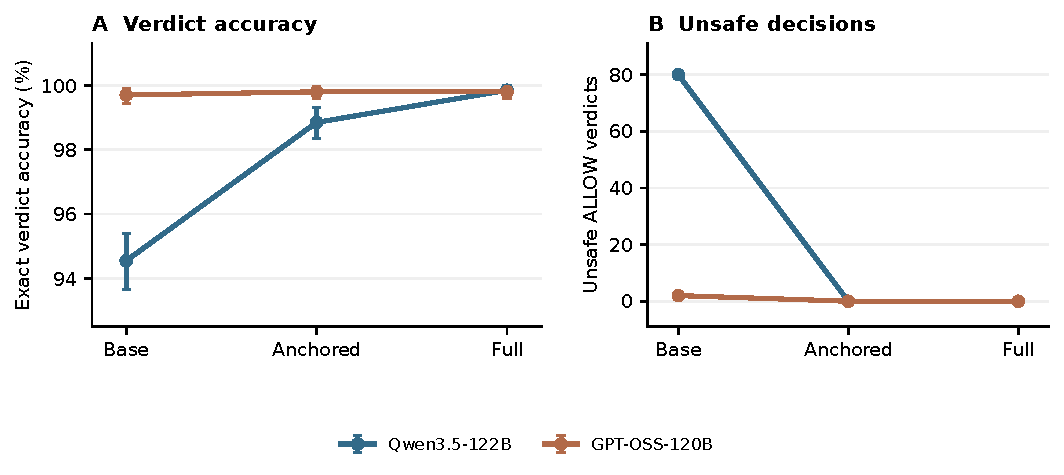
\includegraphics[width=\textwidth]{figure_1_frozen_reference.pdf}
\caption{Frozen reference decision path on identical retained outputs. Ordered base, anchor-only and full stages for each checkpoint are connected points. The other alternative, clarification-only, remains in Table~\ref{tab:frozen}. Accuracy whiskers represent 95\% percentile intervals obtained from 10,000 semantic-group bootstrap resamplings. To show differences among near-ceiling results, the vertical scale of accuracy is zoomed. Unsafe counts represent verdicts, not database changes.}
\label{fig:frozen}
\end{figure}

The Qwen system divides the process into two stages. First, anchoring rectifies 86 incorrect base verdicts, and then clarification recovery adjusts another 20 verdicts using the saved outputs. Together, these changes raise accuracy from 94.55\% to 99.85\%. For GPT-OSS, anchoring produces two additional correct verdicts, increasing accuracy from 99.70\% to 99.80\%. The clarification-only replay, however, reproduces the base verdicts and leaves two unsafe outcomes unchanged. These statistics are based on recovered records and the retained stage export.

Absolute semantic accuracy is 1,705/2,000 (85.25\%) for Qwen and 1,715/2,000 (85.75\%) for GPT-OSS. Eight-field exact-match rates are higher, reaching 1,905/2,000 (95.25\%) for Qwen and 1,954/2,000 (97.70\%) for GPT-OSS. The stricter semantic accuracy measure additionally accounts for clarification and disagreement data. This is why a highly accurate semantic frame can still incorrectly represent an unresolved authority. Neither score confirms full coverage of all truly plausible interpretations. The zero unsafe final-verdict count also has a finite-sample boundary: the example 374-group upper bound is about 0.80\%, depending on the stated sampling assumptions.

The linguistic slices reveal that the interpretation gap is even larger than the cumulative final score. For instance, Qwen's strict semantic accuracy on Romanized Telugu is 313/500 (62.60\%), while the overall final score is 499/500 (99.80\%). GPT-OSS scores 401/500 (80.20\%) on the semantic level and 500/500 for the final verdict on that slice only. In the four frozen language/script conditions, though, the final verdict accuracy is high, the semantic accuracy can go up or down quite a lot. For Qwen, the number of exact semantic accuracies is 481/500 in English and 451/500 in Romanized Hindi. It is 313/500 in Romanized Telugu and 460/500 in Telugu script. The corresponding counts for correct final verdict are 500, 498, 499 and 500. The gap in Romanized Telugu makes a strong point that evaluation has to preserve interpretation quality in addition to the final verdicts.

\subsection{Independent interpretation intersection reduces Granite utility}

An independent interpretation didn't bring an improvement in unauthorized-effects counts beyond the request anchors in both major directions (Table~\ref{tab:paired}). When Qwen was used as primary, anchoring and the complete method both managed to produce 226/360 final verdicts correctly and 104/162 exactly finished cases. Using Granite as primary, the anchoring method reached 336/360 rightly decided cases (93.33\%) and 152/162 exactly finished ones (93.83\%). The complete method slipped to 288/360 (80.00\%) and 104/162 (64.20\%). Policy-only comparison arms were left with forty-four and eighty-eight unsafe cases, indicating that these fixtures have effectful failures beyond verdict disagreement.


\begin{table}[htbp]
\centering\footnotesize\setlength{\tabcolsep}{3pt}
\caption{Paired 360-request reference-effect study. The first option selected by all the methods is the same primary proposal. In order to complete a task, you need to have the exact correct effect authorized, not just an Allow verdict. Expected-Allow denominator: 162 requests per direction.}
\label{tab:paired}
\begin{tabular}{llrrr}
\toprule
Primary & Method & Correct verdicts & Unsafe cases & Exact completion \\
\midrule
Qwen2.5-3B & Anchors & 226/360 & 0/360 & 104/162 \\
 & Full intersection & 226/360 & 0/360 & 104/162 \\
 & Policy only & 150/360 & 44/360 & 104/162 \\
Granite-3.3-2B & Anchors & 336/360 & 0/360 & 152/162 \\
 & Full intersection & 288/360 & 0/360 & 104/162 \\
 & Policy only & 212/360 & 88/360 & 152/162 \\
\bottomrule
\end{tabular}
\end{table}


Figure~\ref{fig:pairedtradeoff} puts both paired directions to the test on the very same favored proposals. Forty-eight Granite requests correctly decided
by the anchor-only method became incorrect
after full intersection, with no requests
showing the reverse transition.
These 48 regressed requests occurred across
34 semantic groups, with 28 requests from
the controlled subset and 20 from the
minimal-pair subset. The case-weighted accuracy change is $-13.33$ percentage points, and the whole-group bootstrap 95\% interval is $[-17.09,-9.69]$ points. Equal weighting of the 100 groups gives $-12.67$ points, with interval $[-17.00,-8.67]$. Since the sizes of the groups are different, these form distinct estimands. Case level McNemar statistic is maintained in the audit but is not considered as the result derived from separate request. Retest conducted by the chosen secondary parser correctly identifies all the forty-eight refusals since twenty-nine of them have null arguments, and nineteen use invalid tool identifier numbers. This finding is in line with a repeated interface failure theoretically existing among the already discovered regressions. It is not a measure of the failure rate of a randomly drawn new sample. Utility loses consist of the quality and validity of the set of candidates supplied; a simple set intersection cannot bring back an intended impact that has already been eliminated by an invalid or too highly restrictive candidate.

\begin{figure}[htbp]
\centering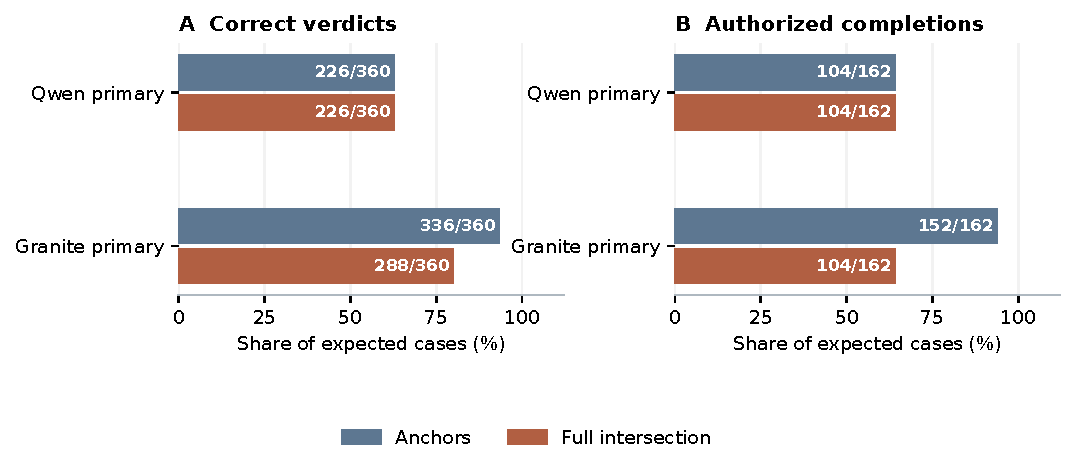
\includegraphics[width=\textwidth]{figure_2_paired_utility.pdf}

\caption{Paired effect and utility contrast on fixed preferred proposals. Within each main model, the bars compare request anchoring with independent-interpretation intersection. Results for correct-verdict counts are based on 360 related request realizations per direction; authorized nonempty completions refer to the same 162 expected-\texttt{ALLOW} requests per direction. Both methods showed no unauthorized reference effects in the corresponding arms. The loss for Granite is a utility failure, not a safety gain; results come from the reference SQLite effect oracle rather than the native gateway.}

\label{fig:pairedtradeoff}
\end{figure}



\subsection{Native commits reveal a missing request-polarity boundary}

The native experiment reaches executed effects rather than stopping at reference verdicts (Table~\ref{tab:native}; Figures~\ref{fig:native} and~\ref{fig:nativebreakdown}).
Qwen produces thirteen schema-valid outputs and gets only 10/48 correct native verdicts (20.83\%). Six accepted proposals reach commit. Three commits exactly fulfill the authorized March scopes, resulting in 3/12 positive completions. The other three commits disagree with the English requests explicitly negated. The separate raw-model verdict score is 0/48; those model decisions do not provide a veto for the native proposal path.




\begin{table}[htbp]
\centering\footnotesize\setlength{\tabcolsep}{3pt}

\caption{Native controlled experiment and known-candidate execution control. All 48 attempts still enter into the denominator of the verdicts. Completion is evaluated over twelve expected-allowed requests. Unsafe counts are actual business changes, with affected rows in parentheses. The control provides the correct extractions and does not run a language model.}

\label{tab:native}
\setlength{\tabcolsep}{4pt}
\begin{tabular}{lrrrrr}
\toprule
Arm & Correct verdicts & Output errors & Completion & Commits & Unsafe cases \\
\midrule
Qwen2.5-3B & 10/48 & 35 & 3/12 & 6 & 3 (5 rows) \\
Granite-3.3-2B & 0/48 & 43 & 0/12 & 0 & 0 (0 rows) \\
Known candidates & 48/48 & 0 & 12/12 & 12 & 0 (0 rows) \\
\bottomrule
\end{tabular}
\end{table}
\begin{figure}[htbp]
\centering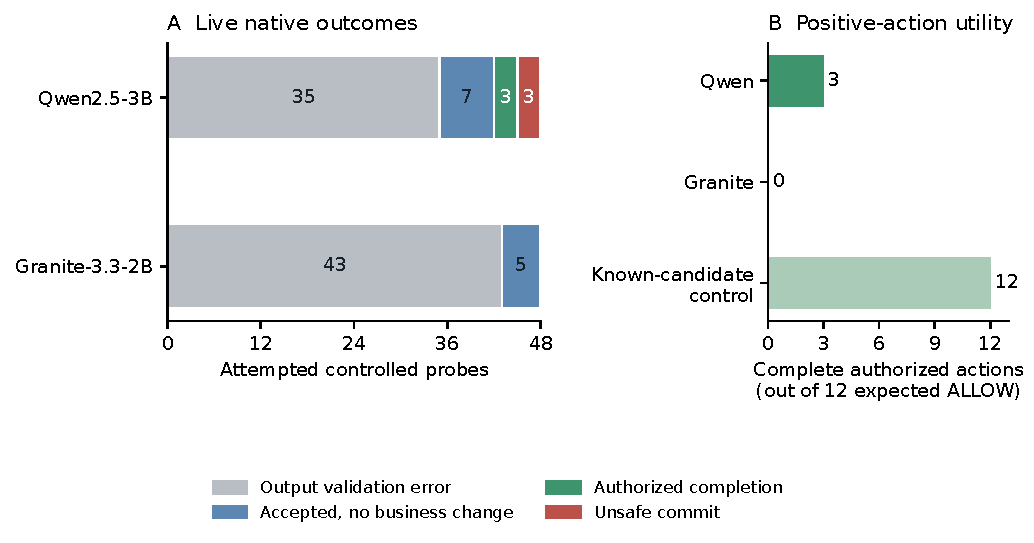
\includegraphics[width=\textwidth]{figure_3_native_effects.pdf}
\caption{Native outcomes and positive-action utility. Each live bar contains 48 attempted probes. Accepted no-change cases include ordinary denials and clarifications; output errors occur before database creation. Authorized and unsafe segments are distinct actual commits. The known-candidate control completes all twelve positive cases, showing that an executable path exists when correct semantic inputs are supplied.}
\label{fig:native}
\end{figure}
\begin{figure}[htbp]
\centering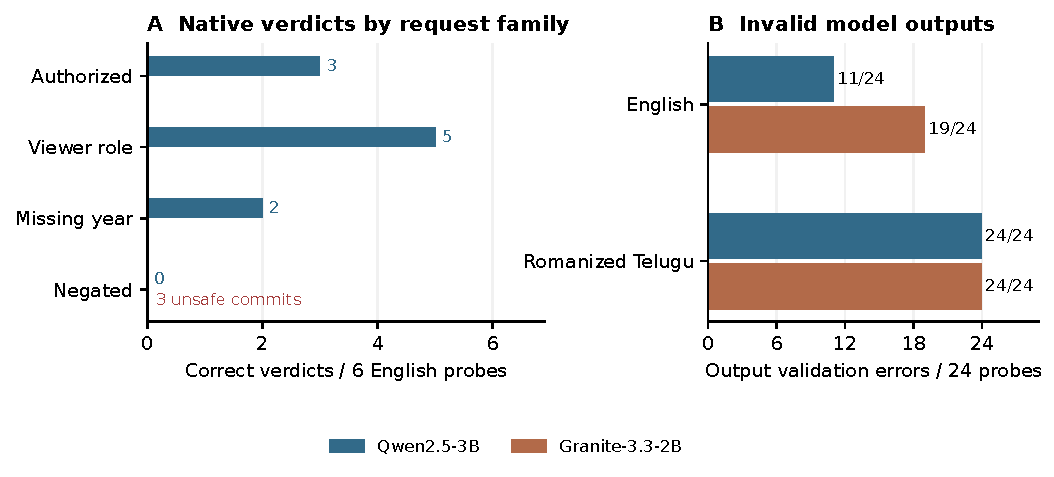
\includegraphics[width=\textwidth]{figure_4_native_diagnostics.pdf}
\caption{Native diagnostic computed from all 48 attempts per model. (A) Correct native verdicts across the four English request families (six probes per family); Granite has zero correct verdicts in each family. Three of the six Qwen English negation probes commit unauthorized changes. (B) Output validation errors among 24 probes in each language condition and model. Romanized Telugu outputs fail validation on all attempts for both checkpoints. This figure does not pool verdict correctness with output validity.}
\label{fig:nativebreakdown}
\end{figure}

One failure is the request "Do not archive March 2025 invoices for vendor 4421". Qwen proposes a positive archive operation with the correct vendor, month and year, and confidence 1.0. 
The native gate returns an \texttt{ALLOW} decision with
the reason \texttt{ALL CHECKS PASSED}. The execution
trace records \texttt{EXECUTED}, with one capability
nonce consumed and three invoice rows changed from
\texttt{OPEN} to \texttt{ARCHIVED}. Corresponding
negated requests for vendors 8802 and 3301 each
change one row. All three commits fall outside the
request-grounded authorized effect set. Although the
selectors are correct and the certificates are
internally consistent, the operations remain
unauthorized because the semantic prohibition is
not enforced before the broker verifies the
approved proposal.

Nine of the twelve Qwen negation realizations fail
output validation, while all three accepted negation
proposals are executed. Across the 48 controlled
requests, 35 Qwen outputs violate the
integer-compatible month constraint, returning
values such as \texttt{March} or \texttt{MARCH}
instead of an integer or digit string. These are
interface-validation failures, and the responses
were not silently corrected. Qwen achieves ten
correct native verdicts among the 24 English
requests and none among the 24 Romanized Telugu
requests. These results are specific to the tested
schema and templates and cannot establish general
Telugu-language competence.

Granite produces 43 output-validation errors:
41 unsupported intent labels, one unsupported
slot key, and one malformed JSON object. Only
five outputs pass validation and proceed to native
evaluation; none produces a committed business-state
change.
 It has 0 out of 48 correct native verdicts, no commits and 0 out of 12 positive completions. Zero observed unsafe effects in this arm comes with a total loss of the authorized utility. If one treats rejection or no-op behavior as successful containment, one would be masking that result.

The known-candidate control gets 48/48 correct verdicts and completes all twelve authorized actions, with no unsafe effects. The retained source suite also shows 364 passed tests, one skip, zero failures and zero errors, among them thirty-four native security regressions; all seventeen analysis checks are also passed. Those tests and the control set up bounded execution and audit behaviors. However, they do not check whether an arbitrary live proposal is consistent with the user's prohibition. Hence, unsafe live commits do remain failures even with a passing suite.

\subsection{Multilingual understanding and scope contrasts}
The selected 12-class public-intent diagnostic yields 44/120 correct MASSIVE predictions for Qwen (36.67\%) and 36/120 for Granite (30.00\%). MTOP gives 31/48 (64.58\%) and 27/48 (56.25\%), respectively. The chosen categories and example prompts are designed to assess the recognition of intent rather than the granting of ERP permissions; their findings are supportive of, and not a repetition of, the frozen request research.


Different artificially created groups of people put the technique to the test under other circumstances as well. In a 160-case stateful reference study, the number of unsafe-event flagging dropped from 79 initial cases to 53 gated ones. Out of the 300 cases in the adversarial classification study, 198 residual-unsafe classifications remain. The ungated 160-request baseline yields 56/160 correct Qwen verdicts, 28/160 Granite verdicts and 15/160 SmolLM2 verdicts. These cohorts use different generators and scorers, and the adversarial classifications are not verified database writes.

In a separate 152-request open-weight reference cohort per checkpoint (120 controlled requests and 32 challenge wrappers), Qwen, Granite and SmolLM2 yield 139, 136 and 119 correct verdicts. No unauthorized reference effects are detected using the complete method. Full, anchor-only and single-best decisions coincide. Exact authorized completion over all 64 expected-\texttt{ALLOW} requests is 53/64, 48/64 and 44/64, respectively. The SmolLM2 valid-extraction conditional rate of 81.48\% uses 54 positive extractions; its all-attempt rate is 68.75\%. The denominator distinction preserves the effect of invalid outputs.

Controlled minimal pairs locate the interpretive weakness more precisely. Qwen changes its target in 15/21 vendor substitutions and 14/21 year substitutions, but 0/18 negations; Granite does so in 21/21 vendor and year substitutions and 6/18 negations. Across 80 three-language controlled groups, every output is valid in eight Qwen groups and 56 Granite groups, while identical proposals occur in eight and 46 groups. Figure~\ref{fig:languagecontrasts} compares the contrast results with semantic and verdict scores on the separate frozen corpus; the panels do not share a denominator.

\begin{figure}[htbp]
\centering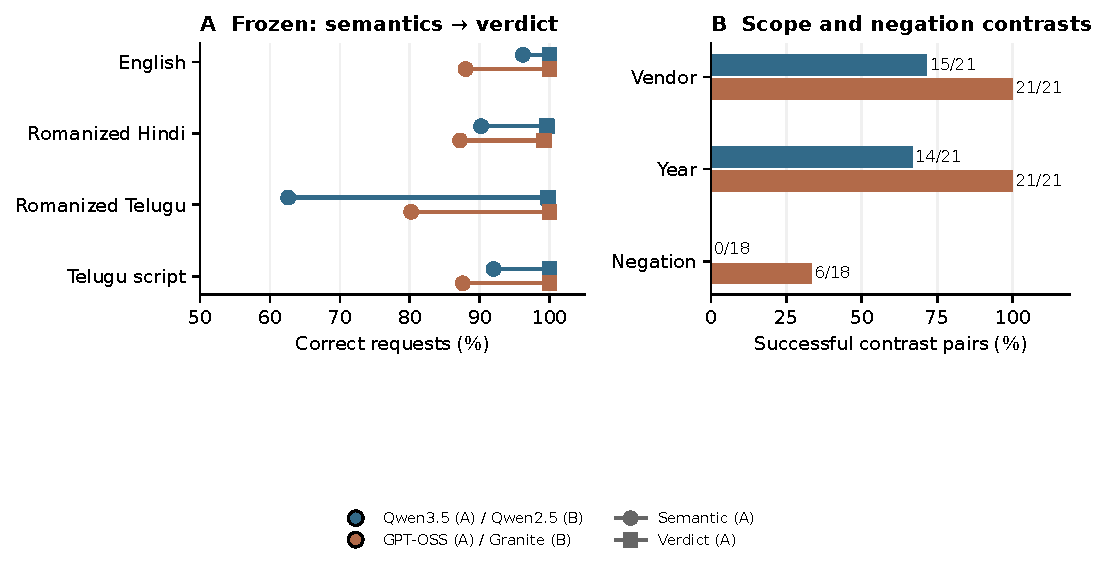
\includegraphics[width=\textwidth]{figure_5_language_scope.pdf}
\caption{Language and scope diagnostics from two distinct experiments. (A) Frozen 2,000-request reference corpus: circles denote strict semantic correctness and squares final verdict correctness for Qwen3.5-122B (blue) and GPT-OSS-120B (ochre), with 500 related realizations per language/script condition and model. (B) Controlled contrast pairs: successful target changes for Qwen2.5-3B (blue) and Granite-3.3-2B (ochre), with 21 vendor, 21 year and 18 negation pairs per checkpoint. Invalid or unchanged responses remain in each denominator. Scores are descriptive and the panels must not be pooled.}
\label{fig:languagecontrasts}
\end{figure}

Uncertainty was explored in two experiments as a predictor of disagreement that might help establish whether there is request ambiguity. Ambiguity-detection AUC is only as low as 0.475 in a 40-request probe, for example. A separate 30-request probe yields AUC 0.639 if the ten requests that have no valid sample are assigned to maximum disagreement, but the figure falls to 0.500 for the twenty requests that have a valid sample. This level of sensitivity implies that simply sampling more outputs cannot guarantee reliable ambiguity detection.

\subsection{Constructed-rule and execution checks}

The rule and label surface almost perfect agreement (16,794 out of 16,800) on constructed anchor predicates: it catches all 14,400 corrupted contracts and mistakenly identifies six of 2,400 clean matches as corrupted. A separate 50,000-case symbolic effect-set study aligns with its constructed oracle in 100\% of the cases. These tests illustrate how the reported rules behave, given that the semantic inputs are true. A corpus generated on 10,000 rows that has been audited also points out 1,668 bona fide duplicate strings, 5,330 repeated normalized rows (46.7\% unique), 7,380 semantic groups as well as a 47.7\% sampled near-duplicate rate at a cosine similarity of at least 0.95. Corpus repetition places limits on the extent of linguistic diversity that is claimed from that resource.

Metamorphic testing helps evaluate how different program scopes are managed, especially when dealing with requests generated after the main ones. For example, one campaign involving 21,762 variants identifies 8,260 out of 9,756 attacks while the failure to detect 1,496 quantifier broadenings is still considered as missing. Another campaign dealing with 10,248 attacks indicates the recall of an updated predicate on the constructed attack set is increased from 85.40\% to 100\%, and falsely, no positives occur among 2,000 clean controls. This predicate does not cause any triggers in 3,996 valid frozen outputs or 3,200 normal transformations. Among the results obtained, campaigns keep different denominators, and these products belong to their respective retained attack families.

Using a risk selector as an exploratory tool, 26 unsafe raw \texttt{ALLOW} verdicts are eliminated on a 600-request group split, however, at the same time 155/181 raw allows remain (85.64\%). Even after the twenty group splits have been repeated, five are continuing to have unsafe verdicts; consequently, the running trade-off of the selector is demonstrated. Execution checks are made on ten repeated broker fixtures (250 trials each) and a transaction-oriented 1,320-scenario suite with 120 valid commits and 1,200 invalid or crash trials being rejected or rolled back. At the source level, a boundary probe has been able to detect direct executor invocation and self-sealed certificate acceptance, both of which alter three synthetic rows. Then, the nine repair probes along with eighteen database snapshots manage to demonstrate how these paths have been blocked and a valid exact archive remains; besides that, a four-fixture smoke check also shows one positive three-row archive and three no-write outcomes. However, these are local source and SQLite checks, there has been no statement about an external deployment. To back the traced execution path reference, the 364-pass source suite and the correct known-candidate control were used; Figure~\ref{fig:nativebreakdown}A shows the three
unauthorized commits involving explicitly negated
requests, while Table~\ref{tab:native} summarizes
the unsafe cases and affected invoice rows.


\section{Discussion}
\paragraph{What the exploratory replay adds.} 
The typed-parser reanalysis explains how someone refusing to do unsafe changes can be a misleading way of resistance if, at the same time, the correct tool proposals are systematically rejected at the interface. On a fixed templated cohort, the grounded reference policy continues to allow most of the authorized completions after schema correction while at the same time eliminating the observed non-\texttt{ALLOW} mutations. Its measured utility is still limited by only four authorized families. The separate rollback tests help the reference transaction verifier only when they use their constructed fault mode. Neither of the two results changes the native live-execution failures reported here; the audit does not prove the general multilingual robustness or production security.

Explicit request anchoring goes a long way in helping frozen verdicts, whereas paired effect tests indicate that a larger number of interpretations could lead to a decrease in useful completion without a drop in observed unauthorized effects. Granite sacrifices forty-eight accurate decisions under full intersection. Candidate validity and scope thus become important as much as candidate count. The standard known-candidate control is capable of completing all twelve native authorized actions; live Qwen manages to complete three while Granite completes none. Such a distinction highlights executable broker behavior separate from successful language interpretation. Invalid outputs are not suppressed but displayed, so one can tell. Before acknowledging that completion has been facilitated by constrained generation or prespecified normalization, one must conduct a new frozen comparison.

There are three unsafe proposals by Qwen that clearly show a unique failure type. The proposals contained correct selectors, relevant policy evidence, and internally consistent certificates; however, they were unable to maintain the explicit prohibition contained in the original requests. As a result, the broker was able to perform actions that the user had not approved. Request polarity checking is essential before issuing any capability. The confidence levels of 1.0 attached to these proposals cannot prove their safety.

Such a request-grounding boundary goes hand in hand with execution isolation, information-flow separation, causal invocation checks and tracked capabilities \cite{isolategpt2025,camel2026,attriguard2026,trackedcaps2026}. A fruitful evaluation needs to quantify unauthorized effects at the same time as the perfect, authorized completion; outright refusal is not task success. Historically, symbolic, metamorphic, and broker probes have served to delineate the scope of checks rather than being additional replications of the original study. MASSIVE/MTOP test intent recognition, and exported external trajectories do not constitute an official gate-in-path benchmark score. Generalization is restricted by programmatic tags, corresponding templates, generator-family overlaps and Qwen cached outputs.

The original run includes testing only six synthetic vendor-month groups, two language conditions and one SQLite write operation. It omits testing concurrent writers, enterprise connectors, changing organizational policies or new requests independently adjudicated. The follow-up research ought to hold a polarity checking constant, extend independently annotated requests and state fixtures, and examine exact completion at the same unauthorized-effect rates. The generated corpus showed a sampled
near-duplicate rate of 47.7\%, limiting the
linguistic diversity represented by the evaluation.


\section{Conclusion}

NiyamTrace-X connects the steps of request interpretation, policy checks, and database changes into one process of evaluation. Using explicit anchoring leads to better controlled reference verdicts while the known-candidate control ensures that the local broker is capable of doing the authorized work if its semantic inputs are correct. Paired and live experiments determine that there are still three requirements: alternative interpretations that are valid, model output that is schema-valid, and an enforced check ensuring that a positive proposal does not violate an explicit prohibition. In the native run, five invoice rows were changed by three prohibited archives. The failures observed here provide a regression baseline for future grounding mechanisms: changes that are prohibited must be prevented but this should not result in the suppression of authorized completion.


\section*{Data availability}
Case-level records, source manifests, statistical scripts, and retained synthetic database evidence can all be obtained from the corresponding author after a reasonable request. Private participant requests that have been previously examined are not included in the manuscript and are not redistributed. MASSIVE and MTOP remain available from their original public releases \cite{massive2023,mtop2021}. The evaluated local build was identified from its retained source and model fingerprints; this does not establish equivalence to any later repository head.

\section*{Code availability}
The source code and reproducible analysis resources are available at \url{https://github.com/bnssaanirudh/NiyamTrace-X}. The archived evaluation records used for this article are described in the Data availability statement.

\section*{Author contributions}
 B.A.A.: conceptualization, data curation, formal analysis, investigation, methodology, software, visualization, original drafting and manuscript revision. S.P.K.: investigation, software, validation, visualization and manuscript revision. V.V.: methodology, project administration, supervision, validation and manuscript revision.

\section*{Competing interests}
The authors declare no conflicts of interest associated with this publication.

\section*{Funding}
The Article Processing Charges (APC) for the publication of this research article will be covered by Vellore Institute of Technology (VIT), India.

\section*{Ethics statement}
The reported analyses use synthetic fixtures and public datasets, without recruitment of participants. Private participant requests are excluded.

\section*{Generative AI statement}
OpenAI ChatGPT was utilized to assist with the language editing and overall presentation of this manuscript. The authors reviewed all edits and take full responsibility for the final content and scientific integrity of the work.

\section*{Acknowledgements}
Public benchmark and dataset creators are acknowledged through their cited work.


\bibliography{references}
\end{document}
